% Chapter Template

\chapter{Non-thermal emission from compact object merger} \label{ch:afterglow} 

In this chapter we discuss models of the non-thermal counterpart 
of the \ac{BNS} mergers, the \ac{kN} afterglow.
%
In Sec.~\ref{sec:intro:afterglow} we recalled the origin of the non-thermal emission, 
and basic methods in calculation of the synchrotron radiation from the expanding into the 
\ac{ISM} \blast{}.
%
We compute the \ac{kN} afterglow light curves via 
semi-analytic, asnisotropic code \pyblast{} 
from the brief description of which we begin the chapter.
%
Then we apply the code \pyblast{} to the dynamical ejecta from our \ac{NR} 
\ac{BNS} merger simulations and investigate how the properties of the 
fast ejecta tail, discussed in Sec.~\ref{sec:bns_sims:fast_de} affect the 
\ac{kN} afterglow and compare our models with recently observed rebrightening 
of \GRB{}.
%
The content of this chapter is based on \citet{Nedora:2021eoj,Hajela:2021faz}.





\section{\pyblast{}}

\def\eq{\text{equation}}
\def\eqs{\text{equations}}

%We calculate the non-thermal 
%radiation arising from the dynamical ejecta propagating into the cold \ac{ISM} 
%with the semi-analytic code \texttt{PyBlastAfterglow}. 
%
We intiialize blast waves using the \ac{NR} ejecta angular and velocity profiles, 
discussed in Sec.~\ref{sec:bns_sims:fast_de}. 
%These take from of the 
%Initial data for the dynamical evolution is taken from the \ac{NR} ejecta 
%profiles for the mass as a function of energy and velocity, that is 
%are used to compute the kinetic energy distributions 
(See Ch.~\ref{ch:bns_sims} and Fig.~\ref{fig:ejecta_vel_hist}).
%
Then, we compute the adiabatic radial expansion of the ejecta in 
the thin shell approximation at each polar angle using the kinetic 
energy distributions.
%
We adopt the \blast{} dynamics formalism from \citet{Nava:2013} that cast the 
Eqs.~\eqref{eq:afterglow:blast} as a set of \acp{ODE} for the \blast{} \ac{LF},
swept-up mass and energy. The system is then solved via 
4th order adaptive step \ac{RK} method.
The effects of radiation losses, discussed in \citet{Nava:2013} and lateral 
spreading of the \blast{}, \citep[\eg][]{Granot:2012} are turned off.
%
The adiabatic index, $\hat{\gamma}$, is computed from the approximation to the 
numerical study of the \trans{} fluid \citep[\eq~5 in][]{Service:1986} as a function 
of normalized temperature \citep[\eq~11 in][]{Peer:2012}. It smoothly connects the 
$\hat{\gamma}=4/3$ and $\hat{\gamma}=5/3$ regimes. 

We adopt a common assumption that a fixed fraction of the \blast{} energy is being
deposited into the electrons, $\varepsilon_e$, and magnetic field, $\varepsilon_B$, 
\citep[\eg][]{Dermer:1997pv}. 
The injected electrons distribution function is Eq.~\eqref{eq:afterglow:elec_dist},
with $p$, the spectral index, being a free parameter.
%
We compute the characteristic \acp{LF}, $\gamma_c$ and $\gamma_m$ using the standard
prescriptions \citep[\eqs~A3 and A4 in][respectively]{Johannesson:2006zs}.

The synchrotron emission in the comoving frame, Eq.~\eqref{eq:afterglow:sync_power},
is approximated with the smooth broken power-law  
\citep[\eqs~A2 and A6 in][respectively]{Johannesson:2006zs}, and the 
the characteristic frequencies are obtained from the characteristic \acp{LF} 
$\gamma_{m}$ and $\gamma_c$ via their \eq~A5.
%
%The synchrotron self-absorption is included via flux attenuation \citep[\eg][]{Dermer:2009}. %
%However, for the applications discussed in this paper, the self-absorption is not 
%relevant as the ejecta remains optically thin for the emission ${\geq3}\,$GHz 
%\citep[\eg][]{Piran:2012wd}.
%

The flux in the observer frame is obtained by itegrating over the \ac{EATS}, 
that are obtained by comping the $t_{obs}$ Eq.~\eqref{eq:afterglow:tobs} for each
segment. The relativist effects are taken into account via 
Doppler factor Eq.~\eqref{eq:afterglow:dop_fac}.
See \citet{Salmonson:2003} for the detailed discussion of the method, 
and \citet{Lamb:2018ohw,Fernandez:2021xce} for the recent implementations


\subsection{Method validation}

In order to validate the code we compare the results obtained with it to the  
published in literature. Specifically, we consider the code designed by \citet{Hotokezaka:2015eja},
and applied to the \ac{BNS} merger ejecta in \citet{Radice:2018pdn}.

\begin{figure}%%[t]
    \centering 
    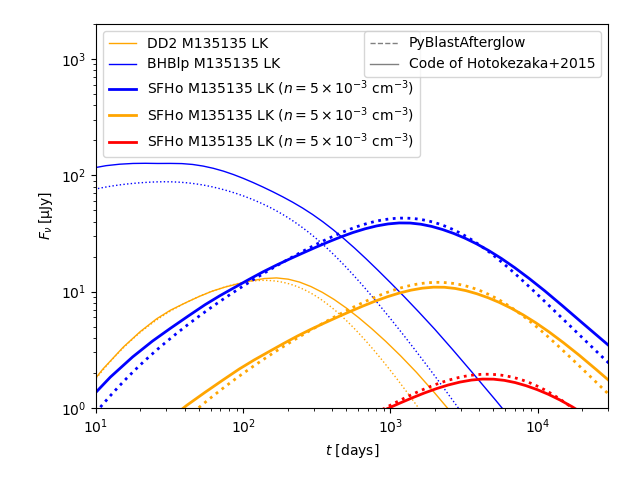
\includegraphics[width=0.49\textwidth]{ejecta_afterglow_vs_hotokezaka.png}
    \caption{
        Cumulative kinetic energy distribution for a selected set of models (\textit{top panel}) 
        and its angular distribution for a BLh $q=1.00$ model (\textit{bottom panel}).
        %% Also shown as a solid black line is the slow quasi-spherical model of \cite{Mooley:2017enz}.
        The vertical light green line marks the $\upsilon_{\text{ej}}=0.6$.
        The top panel shows that equal mass models have a more extend high energy tail,
        while the bottom panel shows that the angular distribution of the ejecta is not 
        uniform.
    } 
    \label{fig:afg_test}
\end{figure}

In Fig.~\ref{fig:afg_test} we show the \ac{kN} afterglow \acp{LC} from 
figures~30 and 31 of \citet{Radice:2018pdn}. The plot shows that that two codes
are in a good agreement. The discpeancies opserved can be attributed for different 
physical treatment of the \blast{} dynamics and synchrotron radiation. 
Notably, considering the large uncertainties on microphysical parameters and 
ejecta properties (discussed below) these discrepancies can be neglected.



\section{\ac{kN} afterglow for \GRB{} rebrightening}


Fig.~\ref{fig:ejecta_vel_hist}. 
Notably, since the largest part (in mass) of the ejecta is equatorial it eludes the 
interaction with the \ac{GRB} collimated ejecta and expands into an unshocked \ac{ISM}.
The latter can decrease the \ac{ISM} density and delay the peak of the 
synchotron emission \citep{2020MNRAS.495.4981M}.
\red{move that to afterglow and rephrase}



\begin{figure*}%%[t]
    \centering 
    %% ---\includegraphics[width=0.49\textwidth]{./figs/scatter_lightcurve_peaks.pdf}
    %% \includegraphics[width=0.48\textwidth]{./figs/xray_obs_representative_all_eos.pdf}
    %% \includegraphics[width=0.48\textwidth]{./figs/radio_obs_representative_all_eos.pdf}
    %% --- \includegraphics[width=0.49\textwidth]{./figs/scatter_q_lam_ideaplot.pdf}
    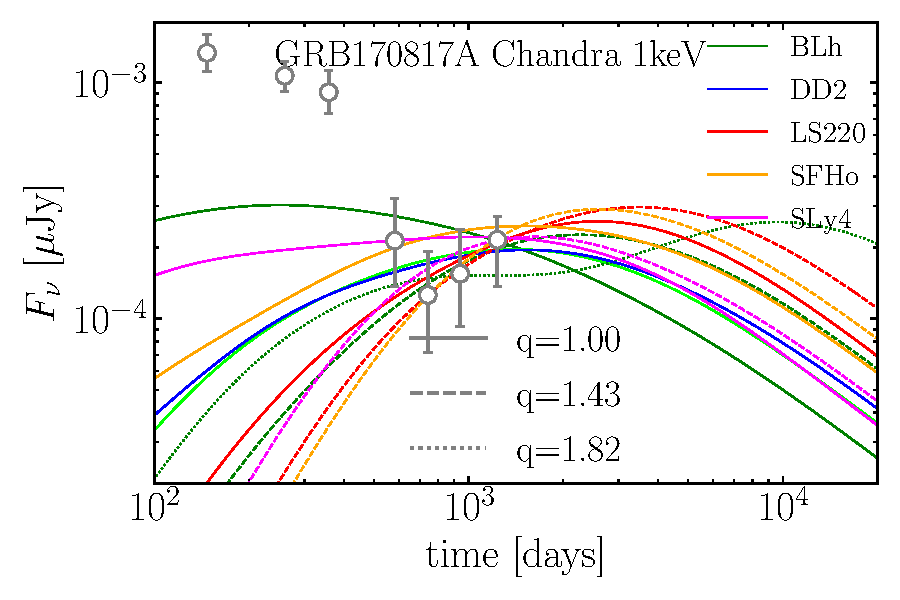
\includegraphics[width=0.48\textwidth]{kn_afterglow/best_xray_obs_representative_all_eos.pdf}
    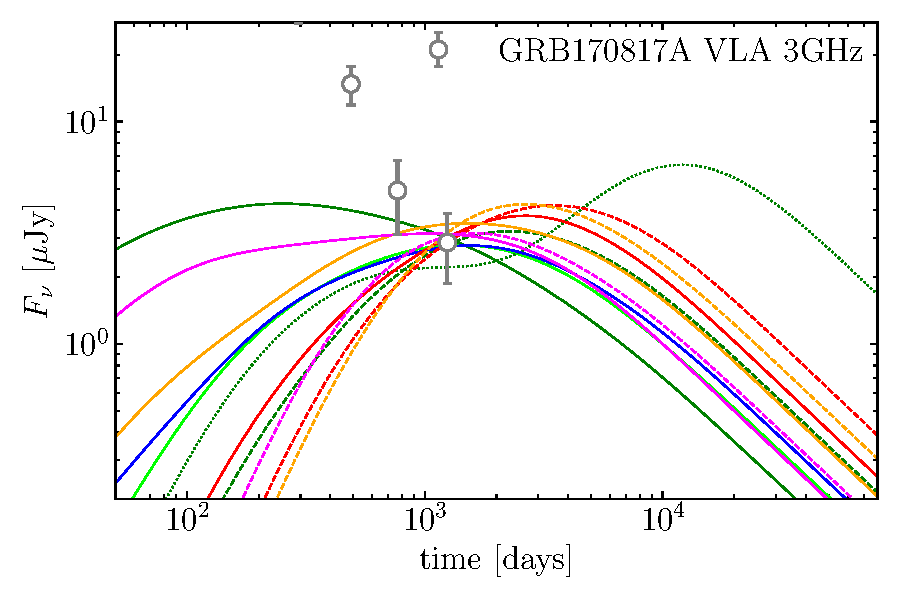
\includegraphics[width=0.48\textwidth]{kn_afterglow/best_radio_obs_representative_all_eos.pdf}
    \caption{
        Representative kilonova afterglow \acp{LC} for \ac{NR} models, 
        in X-ray (\textit{left panel}) and in radio (\textit{right panel}), where 
        %% There, every marker is annotated with two numbers, the tops is the peak time in years and the bottom is the peak flux in nJy ($10^{-9}$~Jy). The red color means that the value is below latest observations, that are $t=3.31$~years and $F_{\nu}=0.34$~$n$Jy. And the green color means that the model peak values are above the observational lower limit. 
        the gray circles are the observational data from \citet{Hajela:2021faz,Balasubramanian:2021kny}.
        %% The gray circles are the observational  in the X-ray band $0.3-10$~keV obtained from \citet{Fong:2017ekk,Hajela:2019mjy,Hajela:2020}.
        The synthetic \acp{LC} are computed with varying 
        micrphysical parameters and \ac{ISM} density within the 
        range of credibility to achieve a better fit to observational data (see Tab.~\ref{tab:pars} for details).
        %% The synthetic \acp{LC} are computed with the following parameters: 
        %% $\epsilon_e = 0.1$, $\epsilon_B\in(10^{-3},10^{-2})$, $n_{\text{ISM}}\in(10^{-3},10^{-2})$~$\ccm{}$.
        %% The last two parameters are varied for each model to achieve a better fit to the data. 
        %% ---
        The plots show that, within allowed parameter ranges, the \acp{LC} 
        from all models are in agreement with observations. 
        Models with moderately stiff \ac{EOS} and $q<1<1.8$ are tentatively preferred,
        as their flux is rising at $t\geq10^3$~days, in agreement with observations.
        %% --- 
        %% The plot shows that while for all models the peak time and magnitude are
        %% relatively close to the X-ray observed data, the models with moderately stiff \ac{EOS} and $q<1<1.8$ are tentatively preferred. 
    } 
    \label{fig:lightcurves}
\end{figure*}

\begin{table}
    \begin{center}
        \caption{
            List of parameters for synthetic \acp{LC} shown in the Fig~\ref{fig:lightcurves} 
            and Fig.~\ref{fig:lightcurve_peaks}.
            For the former the microphysical and \ac{ISM} density are adjusted model-wise 
            to achieved the good agreement with observations. For the latter,
            (the last row of the table) the parameters are the same for all models shown.
            Other parameters, such as observational angle, are the same everywhere (see text).
            (Adapted from \citet{Nedora:2021eoj})
        }
        \scalebox{0.70}{
        \begin{tabular}{l | l l l l}
            Fig~\ref{fig:lightcurves} & $p$ & $\epsilon_e$ & $\epsilon_b$ & $n_{\text{ISM}}$ \\ \hline 
            BLh q=1.00    & 2.05 & 0.1          & 0.002        & 0.005            \\
            BLh q=1.43    & 2.05 & 0.1          & 0.003        & 0.005            \\
            BLh q=1.82    & 2.05 & 0.1          & 0.01         & 0.01             \\
            DD2 q=1.00    & 2.05 & 0.1          & 0.005        & 0.005            \\
            LS220 q=1.00  & 2.05 & 0.1          & 0.01         & 0.005            \\
            LS220 q=1.43  & 2.05 & 0.1          & 0.001        & 0.005            \\
            SFHo q=1.00   & 2.05 & 0.1          & 0.001        & 0.004            \\
            SFHo q=1.43   & 2.05 & 0.1          & 0.01         & 0.005            \\
            SLy4 q=1.00   & 2.05 & 0.1          & 0.001        & 0.004            \\
            SLy4 q=1.43   & 2.05 & 0.1          & 0.004        & 0.005            \\ \hline
            Fig.~\ref{fig:lightcurve_peaks}  & 2.15 & 0.2         & 0.005        & 0.005           
        \end{tabular}
        }
    \end{center}
    \label{tab:pars}
\end{table}

In order to compute the \ac{kN} afterglow \acp{LC}, several free parameters of the model
need to be set. Specifically, we consider the \ac{ISM} density to be uniform with 
$\nism\in(10^{-3}, 10^{-2})\,\ccm$ \citep{Hajela:2019mjy}. 
The observational angle, (the angle between the line of sight and the polar axis of the 
\ac{BNS} system is set to $\theta_{\text{obs}}=30$~deg \citep{TheLIGOScientific:2017qsa}.
The luminosity distance of NGC 4993, the host galaxy of \GW{} is  $41.3\times10^{6}$~pc 
with the redshift $z=0.0099$ \citep{Hjorth:2017yza}.
%
The index of the electron energy distribution, $p$, and microphysical parameters are 
chosed based on the recent observations of the \GRB{}, where the spectral evolution 
was detected \cite{Hajela:2021faz}.  (see however \citet{Troja:2021xsw}). 
%
We consider the 
$\varepsilon_e\in(0.1, 0.2)$,
$\varepsilon_B\in(10^{-3}, 10^{-2})$, 
$p\in[2.05,2.15]$.


In Fig.~\ref{fig:lightcurves} we show the \acp{LC} in X-ray and radio bands for several 
representative \ac{BNS} merger models together with latest \GRB{} observational data. 
%% --- lightcurve shape
Ejecta velocity and angular distribution defines primarily the shape of the \acp{LC}.
Specifically, \ac{BNS} models with ejecta that show broad velocity distribution 
(for example, models with SLy4 \ac{EOS} and $q=1$, shown in Fig.~\ref{fig:ejecta_vel_hist})
leads to a wide \ac{LC}, with an early rise time, comaptible with that of the early \GRB{}
afterglow. This behaviour is guverned by the deceleration of the fastest ejecta shells, 
emission from which peak early. If the velocity distribution is rather narrow, with most 
material moving at ${\leq}0.2$~c (such is the model with LS220 \ac{EOS} and $q=1.43$) 
the \ac{LC} rise is steeper and occurs later (${\sim}10^2$~days after merger). 

%% --- general agreement with observations
Notably, the \ac{kN} afterglow \acp{LC} of most models are in good agreement with the 
rebrightening of the \GRB{} within the uncertain microphsical parameters and \ac{ISM} 
density.
Specifically, this agreement is particularly good for models with moderately stiff 
\acp{EOS} and $1.00<q<1.82$, with respect to the \ac{LC} peak time.

\begin{figure}
    \begin{center}
        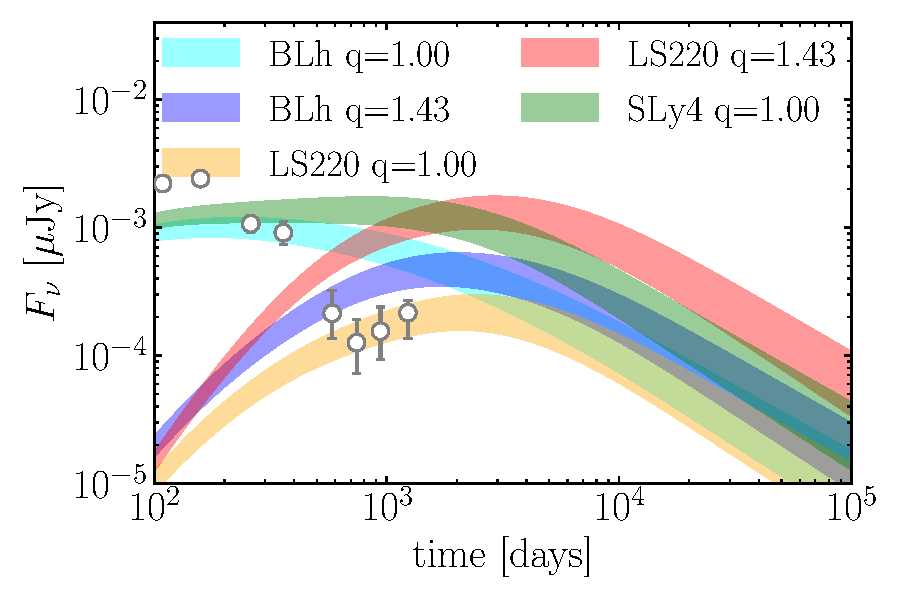
\includegraphics[scale=0.49]{kn_afterglow/KN-afterglow-NR-massratios.pdf}
        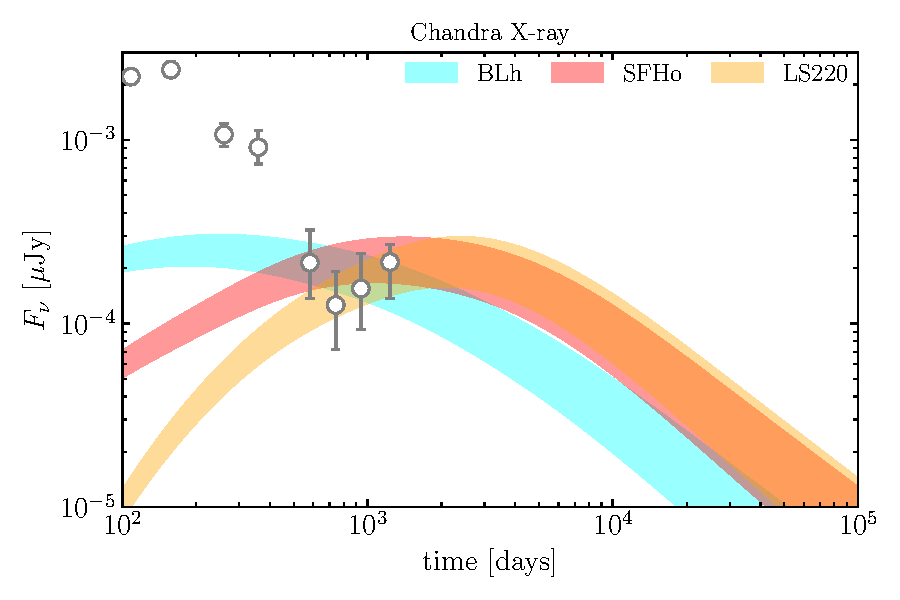
\includegraphics[scale=0.49]{kn_afterglow/KN-afterglow-NR-equalmass.pdf}
        \caption{
            The effect of the cahnging $p$ from $2.15$ (lower boundary of colored bands) to 
            $2.05$ (upper boundary of colored bands) shown in a set of \ac{kN} afterglow 
            X-ray \acp{LC} for \ac{DE} from a sample of \ac{NR} \ac{BNS} merger simulations.
            %% ---
            In \emph{upper panel} the models with different \mr{} are shown and the 
            $\nism=6\times10^{-3}$~cm$^{-3}$, and microphysical parameters, 
            $\varepsilon_{\rm e}=10^{-1}$, $\varepsilon_{\rm B}=10^{-2}$.
            %% --- 
            In \emph{lower panel} the models with $q=1$ are shown and afterglow
            parameters are adjusted to fit observations, 
            with $\varepsilon_{\rm e}=0.1$ fixed and  
            $\nism\sim 6\times 10^{-3}, 5\times 10^{-3},5\times 10^{-3}\,\rm{cm^{-3}}$
            $\varepsilon_{\rm B}\sim 10^{-2},2\times 10^{-3},10^{-3}$ for models with 
            LS220, BLh and SFHo \acp{EOS} respectively.
            (Adapted from \citet{Hajela:2021faz})\red{rephrased}
        }
    \end{center}
    \label{fig:kn_afterglow}
\end{figure}

From the \GRB{} model fitting the electron power law index $p$ is well constrain to $p=2.15$
\citep[\eg][]{Hajela:2019mjy}. The new emergent comonent in \ac{GRB} was found to have a lower 
$p=2.05$ \citep{Hajela:2021faz}. The effect of the decrease in $p$ is shown in 
Fig.~\ref{fig:kn_afterglow}. Notably, the parameters $p$, $\varepsilon_e$. $\varepsilon_b$ and 
$\nism$ are very degenerate, meaining that the change of one can be offset by the change in 
another withing these parameters' ranges of credibility. 

\begin{figure}%%[t]
    \centering 
    %%     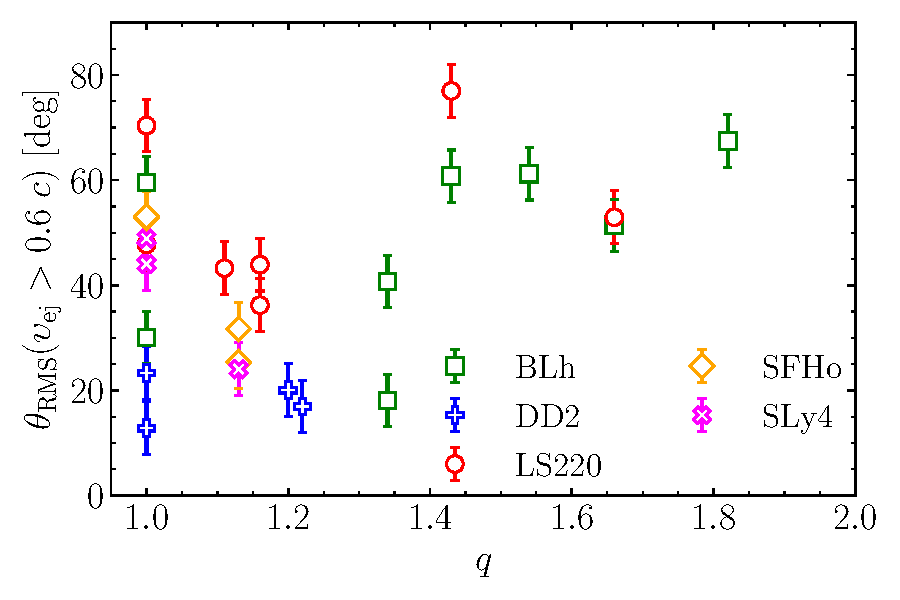
\includegraphics[width=0.49\textwidth]{./figs/scatter_thetarms_vej06.pdf}
    %% \includegraphics[width=0.49\textwidth]{figs/scatter_lightcurve_peaks_vs_lambda.pdf}
    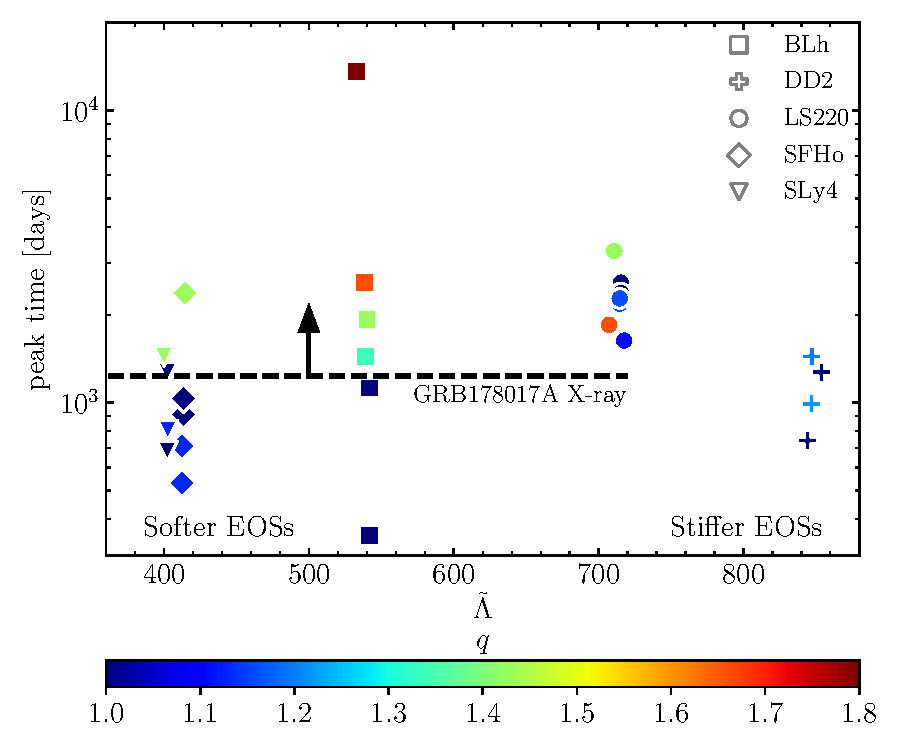
\includegraphics[width=0.49\textwidth]{kn_afterglow/scatter_lightcurve_tpeak_vs_lambda.pdf}
    \caption{
        Peak time, $t_p$, for \ac{LC} for all considered \ac{NR} simulations. 
        Dashed black line corresponds to the last observation of \GRB{} afterglow,
        where the rising flux implies that it is a lower limit on the kilonova 
        afterglow.
        The microphysical parameters and \ac{ISM} density for all models are fixed and 
        given in the Tab.~\ref{tab:pars}.
        The plot shows that in general the $t_p$ increases with mass ration and with 
        softness of the \ac{EOS}, except for the softest, DD2 \ac{EOS}. 
    } 
    \label{fig:lightcurve_peaks}
\end{figure}

%% --- Peak FLUX --- [UPDATED] --- IN CASE IT IS NEEDED [ BUT WITH NO FIGURE ]
If we fix the \ac{ISM} density and microphysical parameters to 
$\nism=5\times10^{-3}$~\gcm, $\varepsilon_e=0.1$ and $\varepsilon_b=5\times10^{-3}$, 
we observe that the \ac{LC} peak flux, $F_{\nu;p}$, is the highest for 
for soft \acp{EOS} such as SLy4. 
In general, however, we do not find a strong dependency between the \ac{EOS} and $F_{\nu;p}$.
With respect to the \mr{} we find that for models with sift \ac{EOS} the larger the \mr{},
the smaller the $F_{\nu;p}$. 
This behaviour can be attributed to the overall dependency of the ejecta mass-averaged 
velocity on the \mr{} (see Fig.~\ref{fig:ejecta:dyn:dsfits}).
As the mass-averaged velocity decreases when \mr{} increases, the 
total kinetic energy budget of these models rises \red{eh?}.
Slower, more massive ejecta have lower peak flux.
Notably, for the models with stiffer \acp{EOS} the dependency on \mr{} is not clear. 

%% --- UNCERTANTIES --- dominant --- microphysics 
%% It is however important to note that the \ac{LC} fluxes and the $F_{\nu,p}$ 
%% depend strongly on the shock michrophsyics. Within the error bars provided by 
%% \citet{Hajela:2019mjy}, they can vary by more then one order of magnitude.  
%% Additionally, the slope of the electron distribution, 
%% $p$, was shown to be lower for the emerging new component of \GRB{} afterglow 
%% (Hajela et al.~in prep). The change from $p=2.15$ to $p=2.05$ translates to the
%% inclrease in $F_{\nu,p}$ by $\sim2$.
%% --- uncertanties -- subdominat -- ejecta
We find that the the \ac{LC} shape and peak time do not depend strongly on the 
uncertain microphysical parameters and \ac{ISM} density. With respect to the latter, 
the peak time changes by a facter of a few when $\nism\in(10^{-3},10^{-2})~\ccm$.
Finite resolution effects that are present in ejecta properties do affect the 
afterglow \acp{LC}. Specifically, the $t_p$ changes by a factor of ${\leq2}$, 
and $F_{\nu;p}$ changes withing a factor of ${\leq4}$. However, our analysis 
shows that the uncertainty in $\nism,\,\varepsilon_e,\,\varepsilon_b$ and $p$ are larger. 
%% --- Robust feature
%% Specifically, the \ac{LC} shape and the peak time appear to be robust 
%% both with resolution and with microphysics, as they set by the dynamics 

%\section{Discussion}
%
%In this section we considered the synchrotron afterglow arising from the interaction 
%of \ac{DE} and \ac{ISM} for a set of \ac{NR} \ac{BNS} models. 
%%
%The recent observations of \GRB{} by Chandra, ${\sim}10^3$~days after the \GW{} event 
%showed the emergence of the rising flux component. Our analysis suggests that this 
%rebrightening can be attributed to the emergence of the \ac{kN} afterglow, as its 
%properties, such as time and flux are naturally reproduced by the \ac{kN} afterglow 
%from ab-initio \ac{NR} \ac{BNS} simulations.
%%
%In the analysis we evolved the \ac{DE} with semi-analytic code and computed its 
%synchrotron emission. 
%We found that the synthetic \acp{LC} are in agreement with the emerging new component 
%in the \GRB{} afterglow within the range of credibility of the microphisycal parameters 
%and of the \ac{ISM} density, $n_{\text{ISM}}$. 
%% The \ac{LC} shape and the time of the peak depends primarily on the 
%% ejecta velocity distribution. If massive fast ejecta component is present, the \ac{LC} 
%% is broader and peaks before $10^3$~days postmerger, while afterglow from 
%% the ejecta with small/absent fast tail peaks on the timescale of $>10^3$~days 
%% (see Fig.\ref{fig:lightcurves}). 

%% --- Note on the observations
%% The latest \GRB{} observations by Chandra \newtxt{(and possibly VLA)} 
%% at $1234$~days show a rising flux (Hajela \textit{et al.} (in prep.)). 

Comparing the \GRB{} observations and synthetic \acp{LC} we observe, that the 
rebrightening at $1243$~days after merger has the following implications:
the \ac{kN} afterglow peak should be (i) later and (ii) brighter than what is
currently observed. 
%
The condition (ii) is weak as the \ac{LC} peak flux is not well constrained due to 
uncertain microphysical parameters.
%% With respect to our models, the (ii) condition suggests that models soft \ac{EOS} and large \mr{} are disfavoured, 
%% as their $F_{\nu,p}$ is lower then the observations.
%% However, an increase in $\epsilon_B$ by a factor of $2$ changes this result.
The condition (i), however, is more robust from that point of view and allows to 
asses afterglow from which models is more supported by observations.

%% --- PEAK TIME 
We show the peak time of afterglow \acp{LC} of all our models in 
Fig.~\ref{fig:lightcurve_peaks}. There, the microphysical parameters and $\nism$ are fixed 
and listed in Tab.~\ref{tab:pars}, last row). 
We consider all models here, including those that do not have fast ejecta tail 
(see Sec.~\ref{sec:bns_sims:fast_de}) as they their ejecta is still energetic enough 
to produce bright afterglow. 
%
The \ac{LC} peak times are ${\sim}10^3$~days for all models that do not undergo the 
tidal disruption. The latter, model with BLh \ac{EOS} and $q=1.82$ produces massive and 
slow ejecta that is cahracteried by a late afterglow \ac{LC} peak ${\sim}10^4$~days.
%
Overall, we observe that the $t_{p}<10^3$~days for models with $q\sim1$ and 
$t_p>10^3$~days for models with larger \mr{}. This relation appears more prominent for 
models with soft \ac{EOS}, as the ejecta in these models has a strong controbution from 
a shocked, fast component when \mr{} is small.
The kinetic energy of the ejecta fast tail increases with the contribution from the 
shocked component. And the afterglow of faster, less massive ejecta peaks earlier 
\citep[\eg][]{Hotokezaka:2015eja}.
Indeed, the time of the \ac{LC} peak depends primarily on the ejecta 
dynamics, the so-called deceleration time \citep[\eg][]{Piran:2012wd}.
%% --- 
%% In the Fig.~\ref{fig:lightcurve_peaks} we show the peak time, $t_{p}$, for each model, 
%% alongside the lower limit (the time of the latest observation).
%% --- 
In Fig.~\ref{fig:lightcurve_peaks} we also show the time of the latest observation 
of the rising flux in \GRB{} (horizontal line). This provides the lower limit on $t_p$
on accordance with (ii).
Synthetic \acp{LC} of models with moderate amount of fast ejecta, \eg, models with 
\acp{EOS} of mild stiffness and \mr{}, lie above the limit, while models with very 
energetic fast tails, found $q=1$ models with very stiff \acp{EOS}, peak earlier. 
%% ---

%%%% <<< moved to overall conclusion >>>
%The main conclusion of our work is that the observed rising flux in the afterglow of \GRB{} 
%at $10^3$~days can be explained by the \ac{kN} afterglow produced by ejecta in 
%ab-initio \ac{NR} \ac{BNS} simulations targeted to \GW{}. 
%%% ---
%Specifically, models with moderately stiff \acp{EOS} and moderately large \mr{}, 
%that produce a mild amount of fast ejecta, are favored.
%%% ---
%Out results are subjected to uncertainties, the dominant among which are introduced 
%by ill-constrained microphysical parameters. 
% Additionally, the systematic effects due to the finite resolution, neutrino treatment 
%and \acp{EOS} might be important. 
%%% ---
%A larger set of observations, that allows for a better assessment of shock microphysics, 
%and a larger sample of high resolution \ac{NR} simulations are required to investigate 
%these uncertainties further. We leave this to future works.